\documentclass{article}

\usepackage{tikz}

%% \AtBeginDocument{\pgfdefobject{mine}{\pgfpoint{2cm}{0cm}}{\pgfpoint{0cm}{2cm}}
%% {\pgfpathcircle{\pgfpoint{0cm}{0cm}}{1cm}
%% \pgfsetfillcolor{red}
%% \pgfusepath{fill}}}

\begin{document}

%\catcode `\^^A 9\relax

A
\textcolor{blue!30!green}{a} 
\begin{pgfpicture}
\pgfpathcircle{\pgfpoint{0cm}{0cm}}{1cm}
\pgfsetfillcolor{blue!30!green}
\pgfusepath{fill}
\end{pgfpicture}
B
\textcolor{blue!30!green}{b} 
\begin{pgfpicture}
\pgfpathcircle{\pgfpoint{0cm}{0cm}}{1cm}
\color{blue!50!green}
\pgfusepath{fill}
\end{pgfpicture}
C
\textcolor{red}{c} 
\begin{pgfpicture}
\pgfpathcircle{\pgfpoint{0cm}{0cm}}{1cm}
\color{green}
\pgfusepath{fill}
\end{pgfpicture}


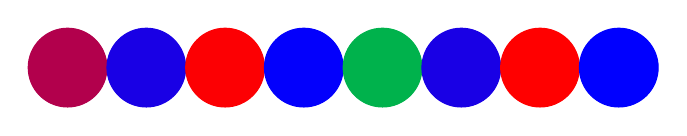
\begin{tikzpicture}
\filldraw[blue!30!red]   (0cm,0cm) circle (0.5cm);
\filldraw[blue!90!red] (1cm,0cm) circle (0.5cm);
\filldraw[blue!1!red] (2cm,0cm) circle (0.5cm);
\filldraw[blue!99!red] (3cm,0cm) circle (0.5cm);
\color{blue!30!green}
\filldraw (4cm,0cm) circle (0.5cm);
\pgfsetfillcolor{blue!30!green}
\filldraw[red!10!blue] (5cm,0cm) circle (0.5cm);
\filldraw[red] (6cm,0cm) circle (0.5cm);
\filldraw[blue] (7cm,0cm) circle (0.5cm);
\end{tikzpicture}

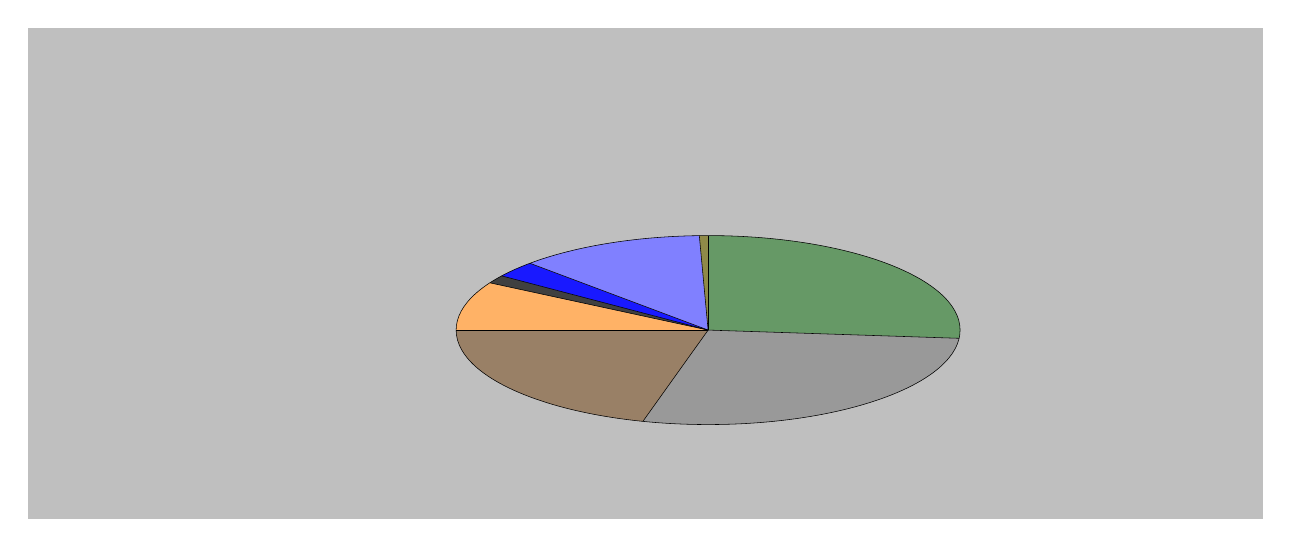
\begin{tikzpicture}
  \begin{scope}[xscale=3.2,yscale=1.2]

    \sffamily
    \coordinate (right border) at (2.0cm,-1.7cm);
    \coordinate (left border)  at (-2.5cm,2.1cm);

    \fill[black!25] ([xshift=-2mm,yshift=1.1cm]left border) rectangle ([xshift=2mm,yshift=-.3cm]right border);

    \fill[green!20!gray]   (0,0) -- (90:1cm) arc (90:-5:1cm);
    \fill[white!20!gray]   (0,0) -- (-5:1cm) arc (-5:-105:1cm);
    \fill[orange!20!gray]  (0,0) -- (-105:1cm) arc (-105:-180:1cm);
    \fill[orange!60!white] (0,0) -- (180:1cm) arc (180:150:1cm);
    \fill[black!75!white]  (0,0) -- (150:1cm) arc (150:145:1cm);
    \fill[blue!90!white]   (0,0) -- (145:1cm) arc (145:135:1cm);
    \fill[blue!50!white]   (0,0) -- (135:1cm) arc (135:92:1cm);
    \fill[yellow!50!black] (0,0) -- (92:1cm) arc (92:90:1cm);

    \begin{scope}[very thin]
      \draw (0,0) -- (90:1cm);
      \draw (0,0) -- (-5:1cm);
      \draw (0,0) -- (-105:1cm);
      \draw (0,0) -- (-180:1cm);
      \draw (0,0) -- (150:1cm);
      \draw (0,0) -- (145:1cm);
      \draw (0,0) -- (135:1cm);
      \draw (0,0) -- (92:1cm);
      
      \draw(0,0) circle (1cm);
    \end{scope}

  \end{scope}    
\end{tikzpicture}




\end{document}
